\subsection{Handling Failures Gracefully}

Another network management consideration for operators is the
occurence of failures (switches, links etc.), which are all too
frequent in datacenter networks~\cite{datacenterfailures}. Failures require
recomputation of paths compliant to the input policies
for the modified topology.  A naive approach is to use \name to
resynthesize the modified instance; However, the new solution may be
drastically different from the original data plane, incurring a large
overhead of removing old rules and installing new
ones~\cite{sdnlatency,updatescheduling}. 
%which could lead to serious
%disruption of tenants' flows.


In what follows, we describe two techniques to handle failures more
gracefully. The first technique is data-plane resiliency (\secref{sec:resiliency}),
which synthesizes and
pre-installs resilient data planes, which even in the event of a
bounded number of link failures, continue to satisfy input
policies. This technique eliminates the need to resynthesize the
forwarding rules for every network failure event, but it 
requires extra backup rules on switches, and it also cannot
capture global operator policies.

Thus, we propose a second mechanism called \emph{minimal repair} (\secref{sec:repair}),
which can transition from the disrupted data
plane to a new policy-compliant one with minimal overhead
 by minimizing the number of
switches whose rule tables are modified. 
Repair does not incur the extra rule cost of the first approach 
and can capture all \Name policies. It is also useful for 
accommodating incremental policy changes, which occur frequently in
cloud datacenters~\cite{mpa-imc15}. The main drawback is that it still
requires removal/installation of rules when a failure occurs, which
can end up being expensive depending on the number of switches
involved.

%% Although the minimal repair mechanism

%% The minimal repair mechanism has two drawbacks: (1) It is {\em reactive}. (2) MaxSMT can be slow to compute a solution impose a high delay to respond to a failure. 
%% cases impose an undue {\em time} overhead in transitioning to the new
%% dataplane.
%% For the new set of policies,
%% \name can use repair to synthesize a new data plane with minimal
%% overhead of installation.



%\name is provided the policies
%and the current forwarding rules $(\overline{Fwd})$ as input. The policy constraints are added as hard
%constraints as described in the earlier sections. To maximize the number of unchanged
%switches, we add \emph{soft} constraints for each switch $sw_1$ of uniform weight as follows:
%Thus, the new forwarding rules $Fwd$ will maximise the number of unchanged
%switch rules in $\overline{Fwd}$, because the constraint will be unsatisfied if a rule on the
%switch changes. 


\subsubsection{Dataplane Resiliency}
\label{sec:resiliency}

%% , and it is crucial to provide
%% certain guarantees during failure scenarios. For example, if the
%% operator wants to guarantee reachability amongst a pair of endpoints,
%% the controller only has to find an active path in the network to
%% re-establish reachability.  However, upon the failure of a link, {\em
%%   reactively} synthesizing a new data plane which satisfies all input
%% policies can be time-consuming, and during this period multiple
%% tenants can suffer from lack of reachability and/or performance
%% issues.  Thus, we propose \emph{policy-compliant resiliency} to tackle
%% network failures by \emph{proactively} synthesizing resilient data
%% planes that even in the event of a bounded number of link failures,
%% continue to satisfy input policies. This eliminates the need to
%% resynthesize the forwarding rules for every network failure event.

In this section, we describe the transformation of input policies to
provide dataplane \emph{t-resilience}~\cite{plinko}, i.e., in the event of
upto $t$ arbitrary link failures, the synthesized data plane still has
a path for each packet class satisfying all policies which is achieved
by synthesizing backup paths that satisfy input policies.  We only
consider reachability, waypoint, and isolation policies in the input.
Global policies like capacity policies and traffic engineering pose a
difficulty in synthesis. For example, consider a packet class $pc$
with a traffic rate of $\sigma(pc)$. By considering the backup paths
with the same traffic characteristics for synthesis, the total traffic
accounted for $pc$ would be $c\times \sigma(pc)$ (for some constant
$c$), leading to under-provisioning of resources. Our current
resilience transformation has no provisions to avoid or minimize the
under-provisioning of resources which affect capacity policies and TE
objectives.
%all backup paths in consideration, while all backup paths will not 
%exist together in the network (backup paths will be deployed during
%a failure event).
%\loris{don't understand previous sentence} \kausik{Have to think!}

Given the physical topology $T=(S,L)$, we define a link-failure
scenario $\theta$ as the set of failed links such that $\theta \subseteq L$.
% For \emph{t-resilience}, we need to
%consider synthesis under any set of $t$ or less arbitrary link failures.
%\begin{mydef}
	We define $\Theta(t)$ as the set of all failure scenarios where no more than $t$
	arbitrary links fail,---i.e. $\Theta(t) = \{ \ \theta \ \ | \ \ |\theta| \leq t\}$.
%\end{mydef}
%We define the projected topology $T^{\theta} = (S, L - \theta)$ as the active 
%physical topology under the failure scenario $\theta$. 	For each class $pc$,
%we construct a data plane graph $\xi = (S, L_{pc})$ for packet class $pc$ from the set
%of paths obtained from the synthesis algorithm. $\xi$
%for class $pc$ over a projected topology $T^\theta$ 
%is resilient if the graph $(S, L_{pc} - \theta)$ has a path from $src$ to $dst$ 
%for the packet class. 
Given a packet class $pc$,
we construct the induced data plane graph $\xi = (S, L_{pc})$ from the links
of the paths returned by the synthesis algorithm for class $pc$.
 For a failure scenario
$\theta$, the active data plane $\xi_\theta = (S, L_{pc} \setminus \theta)$ represents
all the links used by $\xi$ which are unaffected by the failure scenario. A data
plane $\xi$ is {\em resilient} to $\theta$ if it contains a path from the source to 
destination for the packet class in the active data plane $\xi_\theta$.
\begin{mydef}[Resilience]
	A data plane $\xi = (S, L_{pc})$ for class $pc$ is t-resilient if $\xi$ is 
	resilient to all $\theta \in \Theta(t)$.
\end{mydef}
While resilience deals with 
existence of paths during failure scenarios,
we extend the notion to include policy compliance.
\begin{mydef}[Policy-compliance]
	A t-resilient data plane $\xi = (S, L_{pc})$ for class $pc$ is policy-complaint if under
	any failure scenario $\theta \in \Theta(t)$, any path for $pc$ in 
	$\xi_\theta=(S, L_{pc} \setminus \theta)$ satisfies the input policies. 
\end{mydef}
\begin{algorithm}[h]
	\begin{footnotesize}
		\caption{Resilience Transformation}
		\label{restransform}
		\begin{algorithmic}[1]
			\State{[Input] $PC$: Packet classes (Reachability/Waypoint policies)}
			\State{[Input] $I$: Isolation policies (Traffic and Link types)}
			\State{[Input] $t$: Maximum number of arbitrary link failures}
			\State{[Output] $PC^R, I^R$: Transformed set of policies such that the synthesized data
				plane is \emph{t-resilient} and policy-compliant}
			\vspace*{0.25cm}
			\State{$PC^R, I^R \leftarrow \emptyset$}
			\For{$pc:\{src_{pc},dst_{pc},W_{pc}\} \in PC$} 
			\State{// Create $t+1$ edge-disjoint paths of $pc$}
			\State{$\hat{pc} = \{rc_1, rc_2, \ldots rc_{t+1}$\} s.t $\forall m. \ rc_m: \{src_{pc},dst_{pc},W_{pc}\}$} \label{lst:line:respc}
			\State{$PC^R = PC^R \cup \hat{pc}$} 
			\State{$I_{pc} = \{rc_m <> rc_n\ |\ \forall m,n \leq t+1 \wedge m < n\}$}  \label{lst:line:respcisolate}
			\State{$I^R = I^R \cup I_{pc}$} \label{lst:line:respcend}
			\EndFor
			\For{$i: pc_m <op> pc_n \in I$} 
			\State{$\hat{i} = \{ rc_1 <op> rc_2\ | \ \forall rc_1 \in \hat{pc_m}, \forall rc_2 \in \hat{pc_n} \}$} \label{lst:line:respolicy}
			\State{$I^R = I^R \cup \hat{i} $}
			\EndFor \\
			\Return{$PC^R, I^R$}
		\end{algorithmic}
	\end{footnotesize}
\end{algorithm}

\Cref{restransform} shows how \Name can be used to provide \emph{t-resilience}.
The idea is to modify the input policies such that multiple disjoint paths satisfying the original
policies are synthesized for each packet class. 
For \emph{t-resilience}, a packet class $pc$ needs at least $t+1$ edge-disjoint paths from
source to destination. 
We ensure this property holds by creating 
$t+1$ new packet classes ($\hat{pc}$ in line~\ref{lst:line:respc})
and use {\em link-isolation policies} amongst all pairs in $\hat{pc}$ (line \ref{lst:line:respcisolate})
to create $t+1$ edge-disjoint paths for $pc$.
The synthesized data plane $\hat{\xi} = (S, L_{pc})$ for class $pc$ is constructed from the 
paths in the resilient packet class set $\hat{pc} = \{rc_1,\ldots,rc_{t+1}\}$,
i.e., $L_{pc} = \bigcup\limits_{rc \in \hat{pc}} L_{rc}$.  
Each path of $\hat{pc}$ satisfies the reachability policy, 
and any arbitrary $t$ link failure scenario cannot affect all $t+1$ paths.

However, the resilient paths need to satisfy the input isolation policies with other 
packet classes (which themselves have $t+1$ paths for resilience). Thus, for a 
given policy $pc_1 || ~pc_2$, we add isolation policies to every pair of 
classes of $\hat{pc_1}$ and $\hat{pc_2}$ (line \ref{lst:line:respolicy}). This ensures that any path 
chosen in the data planes of $pc_1$ and $pc_2$ will be isolated from one 
another, thus providing policy-compliance under any arbitrary $t-link$ failure
scenario. \Cref{fig:restransform}(a) demonstrates an example transformation for providing $1-resilience$. 

\noindent We now that \Cref{restransform} is sound.
\begin{theorem}[Soundness]
Given input policies $(PC, I)$, 
the data plane $\hat{\xi}_{pc}$ for every packet class $pc \in PC$
 synthesized from
transformed policies $(PC^R, I^R)$  is \emph{t-resilient} 
	and policy-compliant. 
\end{theorem}
\iffull
\begin{proof}
		Assume, $\exists pc$ such that the data plane $\hat{\xi} = (S, L_{pc})$
		is not \emph{t-resilient}. 
		Therefore, there exists a failure scenario $\theta$ such that $|\theta| \leq t$ 
		and $\hat{\xi}_\theta = (S, L_{pc} \setminus \theta)$ 
		is not resilient, i.e., there is no path from the source to destination. 
		Thus, $\theta$ disabled all the paths of $\hat{pc}$. \\
		However, the paths are
		edge-disjoint as each class in $\hat{pc}$ has a link-isolation policy with each 
		other. Thus, $t$ link failures cannot affect $t+1$ 
		edge-disjoint paths of $\hat{pc}$. Thus, $\theta$ disabling all paths of
		$\hat{pc}$ is a contradiction. \\
		Let us consider policy-compliance. Given a failure scenario $\theta \in \Theta(t)$, each data plane $\xi$ of class $pc$ has an active path. Consider a isolation policy in $I$: $pc_1 || \ pc_2$. In line~\ref{lst:line:respolicy} of \Cref{restransform}, each class of $\hat{pc_1}$ will be isolated to
		each class of $\hat{pc_2}$, thus any path of the data planes of $pc_1$ and
		$pc_2$ will satisfy the input policy $pc_1 || \ pc_2$. Hence, the data planes 
		are policy-compliant. 
	\end{proof}
	\fi
\noindent If there are no isolation policies in the input, the resilience transformation in lines 
\ref{lst:line:respc}-\ref{lst:line:respcend} of \Cref{restransform} is complete.
\begin{theorem}[Completeness]
%\loris{What is the input? You should say.
%Given .... such that ...., the synthesized data plane... is....if and only if...}
Given input policies $(PC,I)$ such that $I=\emptyset$,
the synthesized data plane $\xi$ for a packet class $pc$  
is \emph{t-resilient} if and only if it 
contains $t + 1$ edge-disjoint paths from source to destination
for $pc$.
%If there are no isolation policies $I = \emptyset$, 
%	for a packet classes $pc$, the data plane \loris{what dataplane?} is \emph{t-resilient} only if it 
%	contains $t + 1$ edge-disjoint paths for $pc$.
\end{theorem}
\iffull
	\begin{proof}
		We have proved the soundness of the result in \Cref{resiliencesoundness}. 
		Now, let us assume the data-plane $\hat{\xi}$ for $pc$ is \emph{t-resilient} such 
		that less than $t+1$ instances of $pc$ are required for resilience i.e. 
		$|\hat{pc}| < t+1$. Let us consider a 
		t-link failure scenario $\theta, |\theta| = t$ where a link is picked from
		each path of $\hat{pc}$. The active data plane
		$\hat{\xi}_\theta = (S, L_{pc} \setminus \theta)$ will not contain a
		path from source to destination as all paths of $\hat{pc}$ would be disabled.  
		This is a contradiction since $\hat{\xi}$ is \emph{t-resilient}. 
		Therefore, we need atleast $t+1$ instances of $pc$ to ensure \emph{t-resilience}.
		
		Now let us assume there are $t+1$ paths in a \emph{t-resilient} $\hat{\xi}$ for $pc$,
		and not all of them are edge-disjoint. Consider two paths $\pi_1$ and $\pi_2$
		in $\hat{\xi}$ which share a link. We can choose the shared link 
		of $\pi_1$ and $\pi_2$ and $t-1$ links from the other $t-1$ paths 
		and construct a failure scenario $\theta$, $|\theta| = t$.
		The active data plane
		$\hat{\xi}_\theta = (S, L_{pc} \setminus \theta)$ will not contain a
		path from source to destination as all paths of $\hat{pc}$ would be disabled.  
		This is a contradiction since $\xi$ is \emph{t-resilient}. Therefore,
		the $t+1$ paths of $pc$ must be edge-disjoint. 
		
		\noindent Thus, the resilience transformation is sound and complete for a  
		packet class if there are no isolation policies.
	\end{proof}
\fi

%\noindent The transformation demonstrated in \Cref{restransform} is not \emph{complete}
% if the original policies contain link-isolation policies i.e. if the transformed policies
% are unsatisfiable, 
% that does not imply the non-existence of resilient data planes. 
When the original policies contain link-isolation policies, the policies
from \Cref{restransform} may return \texttt{unsat} even when a
resilient data plane exists. Specifically, line~\ref{lst:line:respolicy}
can add additional policies than is required for resilience.
% This is because link-isolation causes edge-disjointness of paths,
% and thus, cannot be both affected by a link failure. 
 \Cref{fig:restransform}(b) shows a transformation required for $1-resilience$ 
 with a smaller number of link-isolation policies among different classes
 of $pc_1$ and $pc_2$ than one obtained from \Cref{restransform}. 
 Consider a failure scenario which disables path
 of $pc_{1A}$. By virtue of the link-isolation policies, $pc_{1B}$ and
 $pc_{2A}$ will be unaffected and can be used as paths for $pc_1$ 
 and $pc_2$ respectively, and $pc_1 <> pc_2$ holds. Now suppose
 $pc_{1B}$ is affected. Similarily, $pc_{1A}$ and $pc_{2A}$ can be used as
 the paths for the original packet classes. The same scenarios hold symmetrically
 for $pc_2$, and thus the resilience transformation can be achieved without
 adding link-isolation policies amongst all the packet classes. 
 
\begin{figure}
	\centering
	\subfloat[Traffic Isolation]{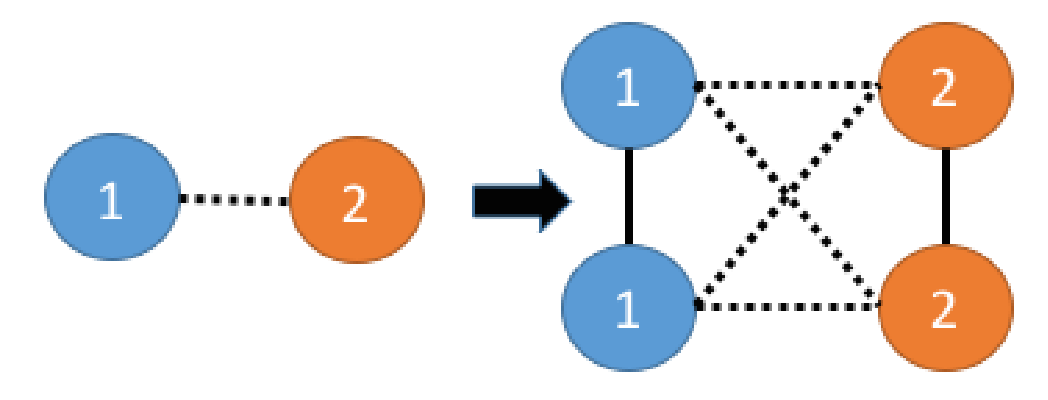
\includegraphics[width=0.5\columnwidth]{figures/resilience.eps}}
	\subfloat[Link Isolation]{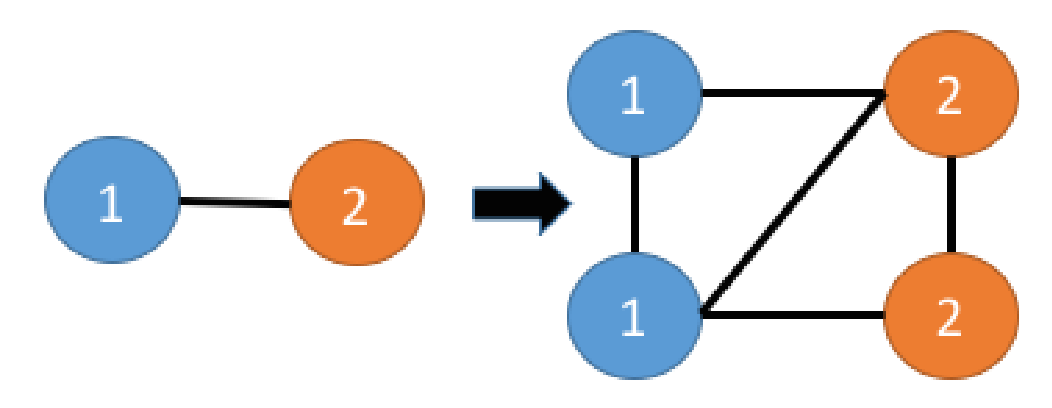
\includegraphics[width=0.5\columnwidth]{figures/resilience-cex.eps}}
	\caption{\label{fig:restransform}
		(a) Resilience Transformation for $pc_1 || \ pc_2$ for providing $1-resilience$. 
		The dotted lines represent traffic isolation policies, 
		while the solid lines represent link isolation. (b) Example of a sufficient transformation
		for 1-resilience in the case of a link-isolation policy.}
\end{figure}

%We presented a sound transformation of policies to provide \emph{t-resilience} in
%the case of reachability, waypoint and isolation policies. Future directions of 
%research involve incorporating capacity constraints and traffic engineering
%for synthesis of resilient data planes and devising a complete transformation for isolation.

\subsubsection{Minimal Repair} \label{sec:repair}
%% Thus, operators need
%% a \emph{network repair} mechanism which can transition with minimal
%% overhead from the current data plane to a policy-compliant one.  This
%% repair mechanism is also useful to accomodate incremental policy
%% changes, which occurs frequently in cloud
%% datacenters~\cite{mpa-imc15}.  For the new set of policies, \name can
%% use repair to synthesize a new data plane with minimal overhead of
%% installation.

Dataplane resiliency impose a high rule storage overhead on switches,
and cannot accommodate global policies like link capacity bounds. 
As an alternative to it, we
extend \name's synthesis algorithm to perform minimal network
repair using MaxSMT.

Formally, the MaxSMT problem is as follows:
given a set of formulas $\Psi_0, \Psi_1, \ldots \Psi_n$ with
associated weights $w_1, \ldots w_n$, find a subset $M \subseteq \{1,
\ldots n\}$ s.t:
\begin{compactenumerate}
	\item $\Psi_0 \wedge \bigwedge_{i \in M} \Psi_i$ is satisfiable.
	\item The \emph{award} $\sum_{i \in M} w_i$  is maximized.
\end{compactenumerate}
The constraints $\Psi_1, \ldots \Psi_n$ denote \emph{soft} constraints, and
the weights $w_i$ encodes the award for including $\Psi_i$ in the satisfying
assignment. 
%The basic intuition is that
%we add the existing configuration as \emph{soft} constraints to the set of \emph{hard} 
%policy constraints. The solver would return a solution which \emph{maximizes} the 
%number of satisfied soft constraints (the older configuration),
%thus resulting in a new policy-compliant forwarding 
%configuration with minimal 
%number of changes from the older one and reducing the overhead of
%updating the forwarding rules in the network.  

We reduce network repair to a MaxSMT problem such that the number of
switches on which rules needs to be updated is minimized. Note that
the disadvantage w.r.t dataplane resiliency is that switches still
require rule updates, which may take time depending on the number of
switches involved.

 Let the policy constraints generated by \name for the new network
 state be $\Psi_0$, and the present data plane be $\overline{Fwd}$
 which does not satisfy $\Psi_0$. The objective is to find new $Fwd$
 which satisfies $\Psi_0$ such that the number of \emph{preserved
   switches} (switches whose rules are unchanged) is maximized. If the
 rules on switch $sw_i$ are preserved, then $Fwd$ and $\overline{Fwd}$
 have the same forwarding rules for all packet classes which traverse
 through $sw_i$. The MaxSMT constraints are described as follows:
\begin{equation}
	\Psi_{sw_i} =  
	  \bigvee_{\mathclap{\substack{\forall sw_j, pc \\
			  		(sw_i, sw_j, pc) \in \overline{Fwd}}}} Fwd(sw_i, sw_j, pc) 
			~~~~~~~~~~~ 
			w_{sw_i}= 1
\end{equation}
By providing $\Psi_0, \Psi_{sw_1}, \ldots, \Psi_{sw_n}$ and associated
weights $w_{sw_1},$ $\ldots w_{sw_n}$ to a MaxSMT solver, we can
synthesize new forwarding rules \emph{minimizing} the number of
switches whose rules have to be changed.  Alternate repair objectives
like minimizing the number of changed forwarding rules can be
expressed similarly. Note that, interestingly, \name's network repair
mechanism described above can also be used to transform an existing
non-compliant network data plane to a policy-compliant one.
